\documentclass[hide notes,intlimits]{beamer}

\mode<presentation>
{
  \usetheme[footline]{UAFshade}
  \setbeamercovered{transparent}
}

% load packages
\usepackage[english]{babel}
\usepackage[latin1]{inputenc}
\usepackage[T1]{fontenc}
\usepackage{lmodern}
\usepackage{pdfpages}
\usepackage{pgfpages}
%\setbeameroption{show notes on second screen=right}

\usepackage{tikz}
\usetikzlibrary{shapes,arrows}
\usetikzlibrary{shadows}

\definecolor{dark red}{HTML}{E41A1C}
\definecolor{dark green}{HTML}{4DAF4A}
\definecolor{dark violet}{HTML}{984EA3}
\definecolor{dark blue}{HTML}{084594}
\definecolor{dark orange}{HTML}{FF7F00}
\definecolor{light blue}{HTML}{377EB8}
\definecolor{light red}{HTML}{FB9A99}
\definecolor{light violet}{HTML}{CAB2D6}

\setbeamercolor{boxed}{fg=black,bg=light blue!25}
\graphicspath{{figures/}}

% Define block styles
\tikzstyle{initialization} = [ellipse, draw, 
    text badly centered, draw=dark violet,
        % The filling: 
        top color=white, 
        bottom color=dark violet]
\tikzstyle{initialization faded} = [ellipse, draw, 
    text badly centered, draw=dark violet!50,
        % The filling: 
        top color=white, 
        bottom color=dark violet!25]
\tikzstyle{hindcast} = [ellipse, draw,
    text badly centered, rounded corners,draw=dark orange,
        % The filling: 
        top color=white, 
        bottom color=dark orange]
\tikzstyle{hindcast faded} = [ellipse, draw,
    text badly centered, rounded corners,draw=dark orange!50,
        % The filling: 
        top color=white, 
        bottom color=dark orange!25]
\tikzstyle{forecast} = [ellipse, draw,
    text badly centered, rounded corners,draw=dark blue,
        % The filling: 
        top color=white, 
        bottom color=dark blue]
\tikzstyle{forecast faded} = [ellipse, draw,
    text badly centered, rounded corners,draw=dark blue!50,
        % The filling: 
        top color=white, 
        bottom color=dark blue!50]
\tikzstyle{arrow line} = [draw, -latex']
\tikzstyle{line} = [draw]

\newenvironment{transbox}[1][]{%
\begin{tikzpicture}
\node[drop shadow,rounded corners,text width=.9\textwidth,fill=white, fill opacity=#1,text opacity=1] \bgroup
}{
\egroup;\end{tikzpicture}} 

\newenvironment{transbox-tight}{%
\begin{tikzpicture}
\node[drop shadow,rounded corners,fill=uaf yellow, fill opacity=0.75,text opacity=1] \bgroup
}{
\egroup;\end{tikzpicture}} 

\newcommand{\jl}{[\![}
\newcommand{\jr}{]\!\hskip 0.003cm ]}
\newcommand{\bpsi}{\boldsymbol{\psi}}
\newcommand{\bPsi}{\boldsymbol{\Psi}}
\newcommand{\bphi}{\boldsymbol{\phi}}
\newcommand{\bPhi}{\boldsymbol{\Phi}}
\newcommand{\bn}{\mathbf{n}}
\newcommand{\bq}{\mathbf{q}}
\newcommand{\bv}{\mathbf{v}}
\newcommand{\D}{\,\mathrm{d}}
\newcommand{\Tsnow}{T_{\text{snow}}}
\newcommand{\Hatm}{H_{\text l}^{\text{atm}}}

\newcommand{\mathtext}[1]{\mathsf{#1}}

% title page
\title[Ice sheet modeling] % (optional, use only with long paper titles)
{Understanding ice sheets through observations and models}
%\subtitle{Understanding ice sheet response to climate change through observations and models}

\author[Aschwanden] % (optional, use only with lots of authors)
{Andy Aschwanden}
% - Give the names in the same order as the appear in the paper.
% - Use the \inst{?} command only if the authors have different
%   affiliation.

% - Use the \inst command only if there are several affiliations.
% - Keep it simple, no one is interested in your street address.

\titlegraphic{\vskip-1.5cm\includegraphics[height=4cm]{grn1km_speed_slr}}

\date{}


\subject{Ice sheet modeling}

\begin{document}


\setbeamertemplate{background canvas}
  {
     \tikz{\node[inner sep=0pt,opacity=1.0] {\includegraphics[width=\paperwidth]{uaf_beamer_shade_bg}};}
} 

% insert titlepage
\begin{frame}
  \titlepage
  \note[item]{I woud like to talk about understanding ice sheets through observations and models}
  \note[item]{In particular I will focus on understanding ice sheet response to climate change}
\end{frame}

\setbeamertemplate{background canvas}
{
%
} 

\setbeamertemplate{background canvas}
  {
     \tikz{\node[inner sep=0pt,opacity=.75] {\includegraphics[height=
\paperheight,width=\paperwidth]{colle}};}
} 

\begin{frame}[plain]
  \begin{transbox}[0.5]
    \begin{block}{What is an ice sheet?}
      \begin{itemize}[<+- | alert@+>] % some control parameters
      \item Artists, Tourists: beautiful landscape
      \item Geographers: element of landscape
      \item Geologists: soft rock, sediment
      \item Hydrologists: water reservoir
      \item Climatologists: subsystem of climate system, climate archive
      \item Physicists: thermomechanical non-Newtonian fluid
      \item Mathematicians: free boundary problem in fluid dynamics
      \item Electrical engineers: one sided accessible dielectric
      \item Glaciologists: part of the cryosphere
      \end{itemize} 
    \end{block}
  \end{transbox}
  \note[item]{Well, before we start talking about ice sheets, we need to ask the question: ``What is an ice sheet''?}
  \note[item]{Depending on who you ask, you may get quite different answers.}
\end{frame}

\setbeamertemplate{background canvas}
{
%
} 



\begin{frame}{The Cryosphere}
  \begin{figure}
    \includegraphics[width=\textwidth]{cryosphere_fuller_projection}
    \\ \scriptsize{source: UNEP Outlook for Ice Sheets}
  \end{figure}
  land ice = \{ ice sheets, ice caps, glaciers\}
  \note[item]{The cryosphere is the frozen part of the terrestrial climate system}
  \note[item]{From the Greek words cryos ``cold'' and sphaira, ``globe''}
  \note[item]{The cryosphere consists of several sub-systems}
  \note[item]{\alert{Ice sheets} are ice masses of continental size (> 50,000 km$^{2}$ e.g. West Virginia) which \alert{rest on solid land}}
  \note[item]{\alert{ice shelves} are the floating extensions of ice sheets, nourished by the adjacent ice sheet}
  \note[item]{land based ice masses smaller than 50,000 km$^{2}$ are \alert{ice caps}}
  \note[item]{smaller ice masses which are constrained by topographic features are \alert{glaciers}}
  \note[item]{\alert{sea ice} floats in the ocean and is formed by freezing ocean water (versus ice shelves are fresh water)}
\note[item]{\alert{lake ice} and \alert{river ice} form similarly}
\note[item]{\alert{Permafrost} is soil that is frozen year round}
\note[item]{ice sheets, ice caps, and glaciers are commonly subsumed as \alert{land ice}}
\end{frame}

\begin{frame}{Land ice}
  \begin{figure}
    \includegraphics<1>[width=\textwidth]{landice_blueglacier}
    \includegraphics<2>[width=\textwidth]{landice}
    \\ \scriptsize{not to scale}
  \end{figure}
  \note[item]{land ice comprises ice sheets, ice caps, and glaciers}
  \note[item]{the two present-day ice sheets, Antarctica and Greenland, \alert{not to scale}}
  \note[item]{Vatnaj{\"o}kull ice cap in Iceland}
  \note[item]{Blue glacier here in Washington}
  \note[item]{of course the Swiss in me wants to show a picture of Gornergletscher}
  \note[item]{What makes glaciers and ice sheets unique is their ability to move.}
\end{frame}

\begin{frame}{Glacier response to climate}
  \begin{figure}
    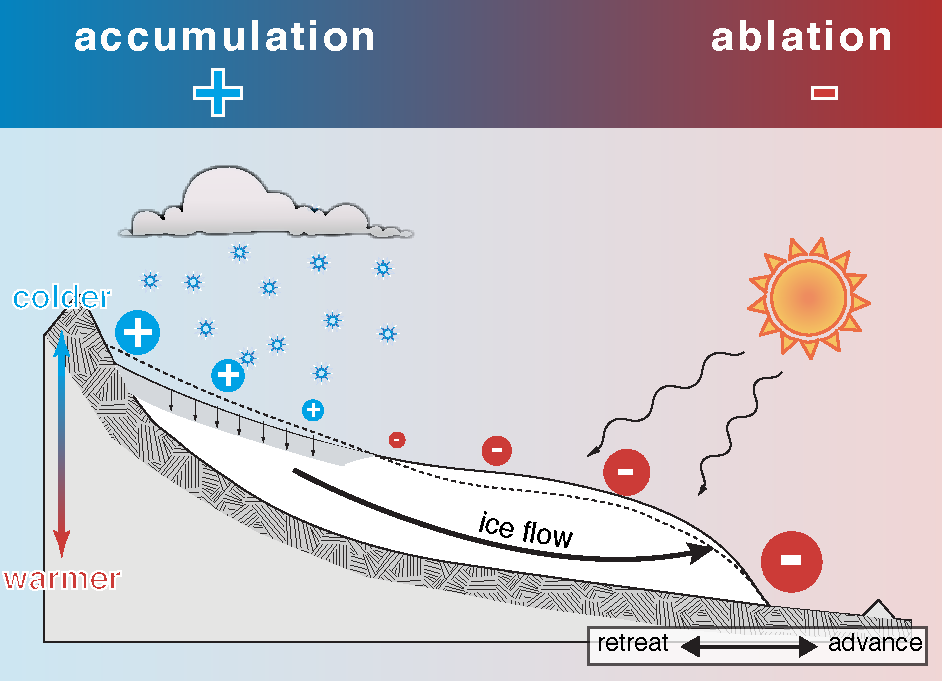
\includegraphics[width=.75\textwidth]{glacier_mb}
  \end{figure}
  \begin{itemize}
    \item glaciers can adjust to changes in climate $\Rightarrow$ stable
  \end{itemize}
  \note[item]{To understand how a glacier or ice sheet responds to climate, let's look at some glacier internals}
  \note[item]{At higher elevation it's generally colder. Precipitation
    falls as snow Snow accumulates. Glaciers begin to form when snow
    remains in the same area year-round, where enough snow accumulates
    to transform into ice. Fluffy snow compacts, it becomes denser, turns into firn,
    and eventually into ice.}
  \note[item]{If we accumulate enough ice, the ice will spread under
    its own weight. It flows down the valley, along the path of least resistance.}
  \note[item]{Ice flow is pretty interesting because ice deforms
    plastically under the influence of gravity. Ice is a non-Newtonian fluid which has a power-law rheology}
  \note[item]{The more ice you have, the more it spreads and the
    faster it flows.}
  \note[item]{ice starts to flow down into lower areas where it is warmer, and starts to melt at the surface}
  \note[item]{if ice melt balances accumulation, the glacier is in equilibrium with its climate, and stays where it is}
  \note[item]{If climate changes the glacier will adjust to the new climate by
    either retreating or advancing, until it finds a new equilibrium}
  \note[item]{As a consequence, glaciers are mostly stable features}
  \note[item]{You can't build an ice sheet of infinite height. That is, the ice will always spread faster than you are able to add new ice on top}
\end{frame}


\begin{frame}[label=ismb]{Ice sheet response to climate}
  \begin{figure}
    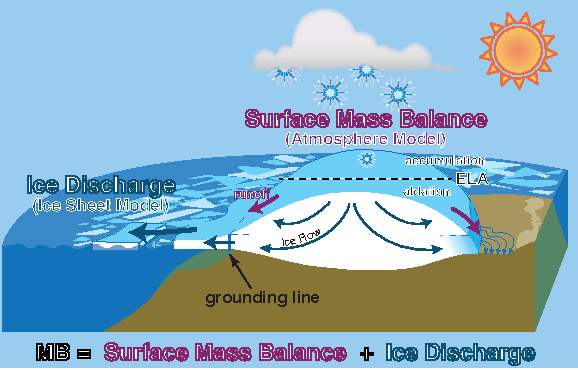
\includegraphics[width=.75\textwidth]{ice-sheet-cartoon}
    \\ \scriptsize{modified from ICESat brochure}
  \end{figure}
  \begin{itemize}
  \item \alert{ice discharge}: vertically-averaged horizontal flow
    velocity $\times$ ice thickness
  \item{50/50 split for Greenland}
  \item{mostly ice discharge for Antarctica}
  \end{itemize}
  \note[item]{Ice sheets respond similarly to climate}
  \note[item]{Melting at the surface is the same process, but ice
    sheets also loose mass by pushing ice into the ocean. This is ice discharge}
  \note[item]{While for Greeenland mass loss is roughly equally split
    by surface melting and by ice discharge, Antarctica looses almost
    all of its mass via calving into the ocean.}
  \note[item]{Another thing sets ice sheets apart:}
\end{frame}


\begin{frame}{Ice sheets really stick out}
  \begin{figure}
    \includegraphics[width=.9\textwidth]{icesheet_topo}
  \end{figure}
  \begin{itemize}
    \item ice sheets rise high enough to create their own weather
  \end{itemize}
  \note[item]{Ice sheets rise high, up to 3 kilometers above sea
    level, and really stick out.}
  \note[item]{they rise high enough to create their own weather.}
\end{frame}


\begin{frame}{Build your own ice sheet}
  \begin{figure}
    \includegraphics[width=.9\textwidth]{ice-sheet-buildup-start}
  \end{figure}
  \note[item]{You can build your own ice sheet from scratch in about 20,000 years.}
  \note[item]{For example Greenland. We start with no ice, and then let it snow and melt at a certain rate}
  \note[item]{At the beginning of the Tertiary, about 65 Mio years ago, the climate was moderate to tropical, and there was no cryosphere}
  \note[item]{Temperatures started to decline and Antartica moved to its current position.}
  \note[item]{About 30 Mio years BP the first Antarctic ice cap started to form, which retreated and advanced many times until to Pliocence (5 Mio BP), where it covered almost all of Antarctica}
  \note[item]{Greenland didn't start to form until 2 Mio BP at the beginning of the Pleistocene Glacial Epoch}
  \note[item]{The cycles of glacials and inter-glacials are mainly controlled by periodic changes in the Earth's orbital parameters, eccentricity, obliquity and precession which influence the seasonal and longitudinal distribution of the solar insolation on Earth}
\end{frame}



\begin{frame}{Ice sheet response to climate}
  \begin{figure}
    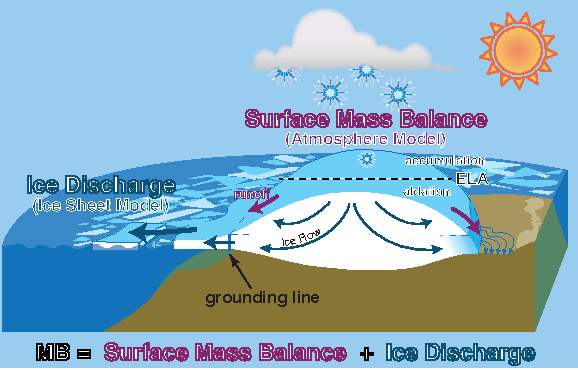
\includegraphics[width=.8\textwidth]{ice-sheet-cartoon}
    \\ \scriptsize{modified from ICESat brochure}
  \end{figure}
  \begin{itemize}
    \item surface processes are reasonably well understood
    \item ice discharge is the wildcard
  \end{itemize}
  \footnotesize{
  \note[item]{Surface mass balance  is reasonably well understood. Higher temperatures lead to increased surface melt, surface lowering, higher temperatures, and so on. This is increased by the albedo feedback. White snow has a high albedo, and reflects most of the incoming solar radiation. If all snow melts, bare ice is exposed. And bare ice has a lower albedo. Therefore less energy is reflected, and more is available for melting. This is a positive feedback.}
\note[item]{I previously said that glaciers are mostly stable. Now there is some concern that, under certain configurations, glaciers may exhibit unstable behavior where small changes lead to a collapse}
  \note[item]{Such an unstable behavior could be triggered at ice sheet's lateral margin.}
  \note[item]{And I will spend the next couple of slides talking about the potential of unstable retreat}
  \note[item]{changes in ocean temperatures and circulation can weaken ice shelves, potentially leading to collapse.}
  \note[item]{ice shelves exert a back pressure and have a buttressing effect. Once gone, there is nothing holding the ice sheet back, we've pulled the plug. It can speed up and deliver ice to the ocean at an increased rate.}
}
\end{frame}


\setbeamertemplate{background canvas}
  {
%
} 


\begin{frame}{Jakobshavn Isbr{\ae}, west Greenland}
 \begin{figure}
    \includegraphics[width=\textwidth]{Jakobshavn_groundline_retreat_wgrn} \\
    \scriptsize{credit: NASA SVS and M. Fahnestock}
  \end{figure}
  \note[item]{As an example, let's look at Jakobshavn Isbr{\ae} in west Greenland}
  \note[item]{Echelmeyer and Harrison found high flow speeds mid-80s but relatively stable behavior}
  \note[item]{In 1997, the glacier suddenly switched from slow thickening to rapid thinning}
  \note[item]{caused by a doubling in subsurface ocean temperature between 1995 and 1998, leading to increased basal melting}
  \note[item]{In summer 1998 the first major increase in surface velocity was seen}
  \note[item]{retreat of the ice front started around 2002}
  \note[item]{now Jakobshavn build only a small floating tongue every
    winter, if at all}
\end{frame}


\begin{frame}{Speed-up of Jakobshavn Isbr{\ae} mid 80's--2008}
  \begin{itemize}
    \item more than doubled its flow speed between the mid-80's and 2008
  \end{itemize}
  \begin{figure}
    \includegraphics[width=\textwidth]{Joughin2004Fig2} \\
    \scriptsize{Joughin et al. (2004)}
  \end{figure}
  \note[item]{illustration of the speed up}
  \note[item]{ice discharge increase from 23 Gt/a in 1996 to 54 Gt/a in 2006}
  \note[item]{Similar behavior has been observed at other outlet glaciers in Greenland}
  \note[item]{Other signs of change}
\end{frame}


\begin{frame}[label=ICESatElevation]{Elevation change between 2003 and 2006}
 \begin{figure}
   \includegraphics[height=7cm]{Greenland_thinning} \vspace{.1em}
   \includegraphics[height=1.25cm,angle=90]{ElevChangeColorBar} \\
    \footnotesize{NASA/Goddard Space Flight Center Scientific Visualization Studio}
  \end{figure}
  \note[item]{pronounced thinning around the ice sheet margins}
\end{frame}


\begin{frame}
  \frametitle{Ice Cloud Land Elevation Satellite (ICESat)}
  \vspace{-2em}
  \begin{columns}[c]
    \begin{column}{.85\linewidth}
    \begin{figure}
      \includegraphics<1>[width=.9\textwidth]{icesat-pov} \\
    \end{figure}
    \end{column}
    \begin{column}{.15\linewidth}
    2003--2009
    \begin{figure}
       \includegraphics<1>[width=\textwidth]{ICESat_logo} \\[2em]
       \includegraphics<1>[width=\textwidth]{icesat-satellite}
    \end{figure}
    \end{column}
  \end{columns}   
  \begin{center}
    \footnotesize{credit: NASA Goddard Space Flight Center}
  \end{center}
  \note[item]{Geoscience Laser Altimeter System (GLAS) scans the surface repeatedly to detect elevation changes}
\end{frame}


\begin{frame}
  \frametitle{Gravity Recovery and Climate Experiment (GRACE)}
    \begin{figure}
       \includegraphics<1>[height=3.7cm]{grace-satellites} \hspace{2em}
       \includegraphics<1>[height=3.7cm]{grace-trend} \\
       \footnotesize{courtesy of A. Arendt}
     \end{figure}
  \begin{itemize}
  \item precise measurements of orbital variations of tandem satellites are used to construct time variable gravity field
  \end{itemize}
\end{frame}


\begin{frame}{Global mass changes observed by GRACE}
  \begin{figure}
    \includegraphics[width=\textwidth]{grace-world} \\
    \scriptsize{credit: A. Arendt, S. Luthcke, modified}
  \end{figure}
  \note[item]{largest mass changes occur along Greenland's perimetry, the West Antarctic Ice Sheet, and Alaska}
\end{frame}


% \begin{frame}{Marine Ice Sheet Instability}
%   \begin{figure}
%     \includegraphics[height=6cm]{vaughan2007_misi} \\
%     \scriptsize{Vaughan \& Arthern (2007)}
%   \end{figure}
%   \note[item]{largest mass changes occur along Greenland's perimetry, the West Antarctic Ice Sheet, and Alaska}
% \end{frame}


\begin{frame}{Antarctica}
  \begin{figure}
    \includegraphics[width=9cm]{bamber2009_misi} \\
    \scriptsize{modified from Bamber et al (2009)}
  \end{figure}
  \begin{itemize}
  \item WAIS is potentially unstable
  \item could raise global mean sea level by $\sim$3\,m
  \end{itemize}
  \note[item]{We now move to Antarctica}
  \note[item]{Theoretical work since the 1970's suggests that the West Antarctic Ice Sheet is potentially unstable as a consequence of the Marine Ice Sheet Hypothesis}
  \note[item]{In short, MISI is the hypothesis that the loss of buttressing ice shelves leads to a rapid and irreversible retreat of the ground line where the bedrock elevation is below sea level and slopes upward towards the ocean.}
  \note[item]{WAIS is very unique, as it possess a large area where these conditions are met}
  \note[item]{loss of WAIS could raise global mean sea level by about 3 meters or a bit more.}
\end{frame}


\setbeamertemplate{background canvas}
  {
     \tikz{\node[inner sep=0pt,opacity=1] {\includegraphics[height=
\paperheight,width=\paperwidth]{sea_level_rise_graph}};}
} 


\begin{frame}{Why we care}
\note[item]{The questions raised in the previous slides are interesting not only for pure scientific reasons}
\note[item]{but rising sea level will also have social and economic implications}
\note[item]{tide gauge records and satellite altimetry show that sea level is steadily on the rise}
\note[item]{mostly due to thermal expansion and melting glaciers and ice sheets}
\end{frame}

\setbeamertemplate{background canvas}
  {
     \tikz{\node[inner sep=0pt,opacity=1] {\includegraphics[height=
\paperheight,width=\paperwidth]{sea_level_rise_icedynamics}};}
} 


\begin{frame}{Why we care}
  \note[item]{so far, sea level closely followed global mean temperature}
  \note[item]{However, sea level rise could rise much faster in the future if ice dynamics goes wild, as explained in the previous slides}
\end{frame}


\setbeamertemplate{background canvas}
  {
     \tikz{\node[inner sep=0pt,opacity=1] {\includegraphics[height=
\paperheight,width=\paperwidth]{sea_level_rise_composite}};}
} 


\begin{frame}{Why we care}
  \note[item]{probably all of us have seen renderings like these here about our potential future}
  \note[item]{But how likely is it to happen?}
\end{frame}


\setbeamertemplate{background canvas}
  {
     \tikz{\node[inner sep=0pt,opacity=1] {\includegraphics[height=
\paperheight,width=\paperwidth]{flooding}};}
} 


\begin{frame}{Why we care}
  \begin{transbox}[0.75]
      \begin{itemize} 
        \item mitigation and adaptation efforts require long-term planning
        \item appropriate measures depends on projected sea-level rise
        \end{itemize}
  \end{transbox}
\end{frame}


\setbeamertemplate{background canvas}
  {
     \tikz{\node[inner sep=0pt,opacity=.5] {\includegraphics[height=
\paperheight,width=\paperwidth]{nasa-jako-front-apr-2012_credit}};}
} 


\begin{frame}{Why we need ice sheet models}
  \begin{transbox}[0.75]
    ``Realistic projections of ice sheet response to a changing climate
    should be based on a physical understanding of the processes involved,
    rather than trend extrapolation of historical observations'' (Arthern
    \& Hindmarsh, 2006)
  \end{transbox}
  \note[item]{To estimate the sea-level response of ice sheets to
    climate change, we need ice sheet models}
\end{frame}


\setbeamertemplate{background canvas}
{
%
} 


\begin{frame}{What is an ice sheet model?}
  \begin{figure}
    \includegraphics<1>[width=9cm]{grn_system_eqns}
  \end{figure}
  \begin{columns}[c]
    \begin{column}{.40\linewidth}
      \begin{itemize}
      \item ice dynamics
      \item thermodynamics
      \item surface processes
      \end{itemize}
    \end{column}
    \begin{column}{.55\linewidth}
      \begin{itemize}
      \item boundary conditions
      \item hydrology
      \item ice-ocean interaction (e.g. calving)
      \end{itemize}
    \end{column}
  \end{columns}
  \note[item]{An ice sheet model solves numerical approximations to the balance equations of mass, momentum}
  \note[item]{Ice flow is governed by Stokes equations with a power-law rheology}
  \note[item]{Because the viscosity of ice strongly depends on the thermal state, we also need to solve an energy balance equation}
  \note[item]{This makes the problem thermomechanically-coupled.}
  \note[item]{some processes such as hydrology are currently only parametrized}
\end{frame}


\begin{frame}{Why ice sheet modeling is easy}
  \begin{figure}
    \includegraphics<1>[width=9cm]{grn_system_eqns}
  \end{figure}
  \begin{itemize}
  \item composed of a single, largely homogenous material
  \item flow governed by the Stokes equations known since the mid-19th century
  \item flows slowly: we can ignore turbulence, Coriolis and other inertial effects
  \end{itemize}
\end{frame}


\begin{frame}{Why ice sheet modeling is so hard}
  \begin{figure}
    \includegraphics<1>[width=9cm]{grn_system_eqns}
  \end{figure}
  Specifying the stress boundary condition at the
  \begin{itemize}
  \item seaward margin
    \item base
  \end{itemize}
  is challenging.
\end{frame}


\begin{frame}{Challenge: ice base}
  \begin{columns}[c]
    \begin{column}{.50\linewidth}
      \begin{figure}
        \scriptsize{basal resistance} \\
        \includegraphics[width=\textwidth]{tauc}
      \end{figure}
    \end{column}
    \begin{column}{.5\linewidth}
      \begin{itemize}
      \item stresses vary by orders of magnitude
      \item transience and complexity of basal water flow
      \item despite more than 5 decades of research, we only have crude parametrizations
      \end{itemize}
    \end{column}
  \end{columns}
  \note[item]{First, stresses at the base vary by several orders of magnitude}
  \note[item]{depend on many factors, most importantly on the presence or absence of water}
  \note[item]{basal hydrology (the glacier's plumbing system) runs on a faster time scale than the ice flow itself}
  \note[item]{but the sub-glacial environment is not easy accessible}
  \note[item]{at the basal boundary, interactions between water flow, friction, heat flow, and sediment deformation is so complex that a deriving a theory from first principles is real challenge}
\end{frame}


\begin{frame}{Challenge: seaward margin}
      \begin{figure}
        \includegraphics[width=.75\textwidth]{ice-shelf}
      \end{figure}
      \begin{itemize}
      \item ocean circulation $\Rightarrow$ basal melt rates
      \item calving mechanism
      \end{itemize}
      \note[item]{a big challenge is to understand how changing ocean currents and ocean temperatures affects sub-shelf basal melt rates}
      \note[item]{how this can weaken a shelf, and potentially lead to break up}
\end{frame}


\begin{frame}{IPCC and ice sheet models}
  \begin{beamercolorbox}[rounded=true,shadow=true]{boxed}
    \begin{block}{IPCC (2007), Box 4.1: Ice Sheet Dynamics and Stability}
      ``\ldots but recent changes in ice sheet margins and ice streams cannot be simulated accurately with these models, \ldots.''
    \end{block}
  \end{beamercolorbox}
  \vspace{1em}
  \begin{itemize}
  \item the above statement received lots of attention
  \item triggered projects such as SeaRISE (Sea Level Response to Ice Sheet Evolution) and ice2sea
  \end{itemize}
\end{frame}


\begin{frame}{Ice Sheet Models, 2007--}
      \begin{figure}
        \includegraphics[width=.95\textwidth]{ism}
      \end{figure}
      \note[item]{Since the last IPCC report, new ice sheet models have emerged, such as ISSM from JPL, ElemerICE developed in Finland and France, and the Parallel Ice Sheet Model, from Fairbanks and Germany}
\end{frame}


\begin{frame}{Ice Sheet Models, 2007--today}
      \begin{figure}
        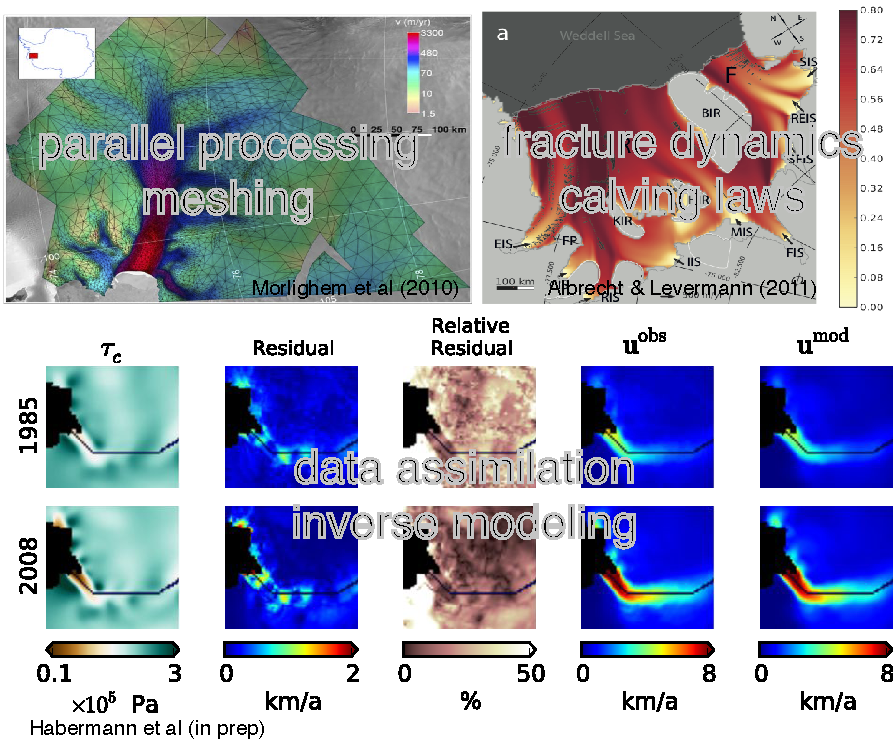
\includegraphics[height=8cm]{newsince2007}
      \end{figure}
      \note[item]{we now have parallel processing and better meshing techniques which allow to resolve rapidly-changing areas}
      \note[item]{improvements on the seaward margin: fracture dynamcis and physically-based calving laws}
      \note[item]{at the base: we use data assimilation techniques and inverse methods to estimate basal properties}
\end{frame}


\begin{frame}{A word of caution}
 \begin{figure}
   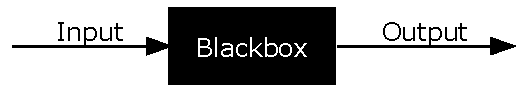
\includegraphics[height=1.25cm]{blackbox}
\end{figure}
\begin{itemize}
  \item ice sheet models should not be used as a ``black-box''
  \item require serious modeling choices (physics, physical and
numerical parameters, etc) based on glaciological knowledge
  \item \alert{``garbage in $\Rightarrow$ garbage out''}, sometimes
\alert{``garbage in $\Rightarrow$ gospel out''}
  \item a model is only as good as the input data (at best)
 \end{itemize}
 \begin{figure}
  \includegraphics[height=2.5cm]{gigo}
 \end{figure}
\end{frame}


\begin{frame}{Ice Sheet Models, 2007--today}
      \begin{figure}
        \includegraphics[width=\textwidth]{speed_sar_today_grace}
      \end{figure}
\end{frame}


\begin{frame}{Modeling in 1995 and today}
  \begin{figure}
    \includegraphics[width=\textwidth]{speed_sar_eismint_today}
    \\ \scriptsize{a) observed \qquad b) model 1995 \qquad c) model 2013}
  \end{figure}
\end{frame}


% \begin{frame}{Ready for the future?}
%   \begin{figure}
%     \includegraphics[width=\textwidth]{ts_RCP45_imass}
%   \end{figure}
% \end{frame}


\begin{frame}{Ready for the future?}
  \begin{figure}
    \includegraphics[width=.85\textwidth]{sea_level_rise}
  \end{figure}
  \begin{itemize}
  \item we now have decent numerical ice flow models
  \item but we need uncertainty quantification
  \end{itemize}
\end{frame}

% \begin{frame}{In the next five years}
%   \vspace{0.5em}
%   \begin{block}{Observations}
%     \begin{itemize}
%     \item sub-shelf basal melt rates
%     \end{itemize}
%   \end{block}
%   \begin{block}{Theory}
%     \begin{itemize}
%     \item grounding line migration
%     \end{itemize}
%   \end{block}
%   \begin{block}{Models}
%     \begin{itemize}
%     \item coupling to ocean and climate models
%     \end{itemize}
%   \end{block}
%   \note[item]{  What we need to do to arrive at more reliable predictions of the contribution of ice sheets to sea level:
% }
% \end{frame}


\end{document}